\section{Storage Components}
\label{sec:storage}

In this section, we illustrate the design of our storage components. We begin by listing all the components in our design, followed by a demonstration of how each component interacts with the others.

\subsection{Data Components} 
\label{subsec:data-components}

The data components primarily consist of the following objects:

\begin{itemize} 
    \item \textbf{BlockData}: This object stores the actual data. The data is stored as an array of bytes, with the size determined by the block size of different computers. 
    \item \textbf{BlockPtr}: This object points to the position of the \texttt{BlockData}. Given a file stream, the \texttt{BlockPtr} can access a specific range of positions within that file stream. 
    \item \textbf{DataPtr}: This object points to a specific range of positions within a \texttt{BlockData}. In real-time operations, a \texttt{BlockPtr} is used to manage the loading and storing of the \texttt{DataPtr}. 
    \item \textbf{Record}: A \texttt{Record} is a subclass of the \texttt{DataPtr}. It can access a specific range within the \texttt{BlockPtr}, corresponding to the size of the record.
    \item \textbf{Schema}: The \texttt{Schema} manages the field names and data types of a table. A Schema object is used to determine the number of bytes required to write input data and the number of bytes needed to read a record when loading from an array of bytes.
\end{itemize}

During the reading and writing processes, all data is converted into a uniform format, specifically an array of bytes. For example, an int or float data type is converted into an array of size 4 bytes, while a bool data type is converted into an array of size 1 byte. During reading, we access only the \texttt{BlockPtr} or \texttt{RecordPtr}, which points to a specific location in the data. When a specific range is needed, the corresponding byte array is loaded into memory. A detailed illustration of our storage format and components is provided in ~\Cref{fig:storage-component}.

\begin{figure}[t]
    \centering
    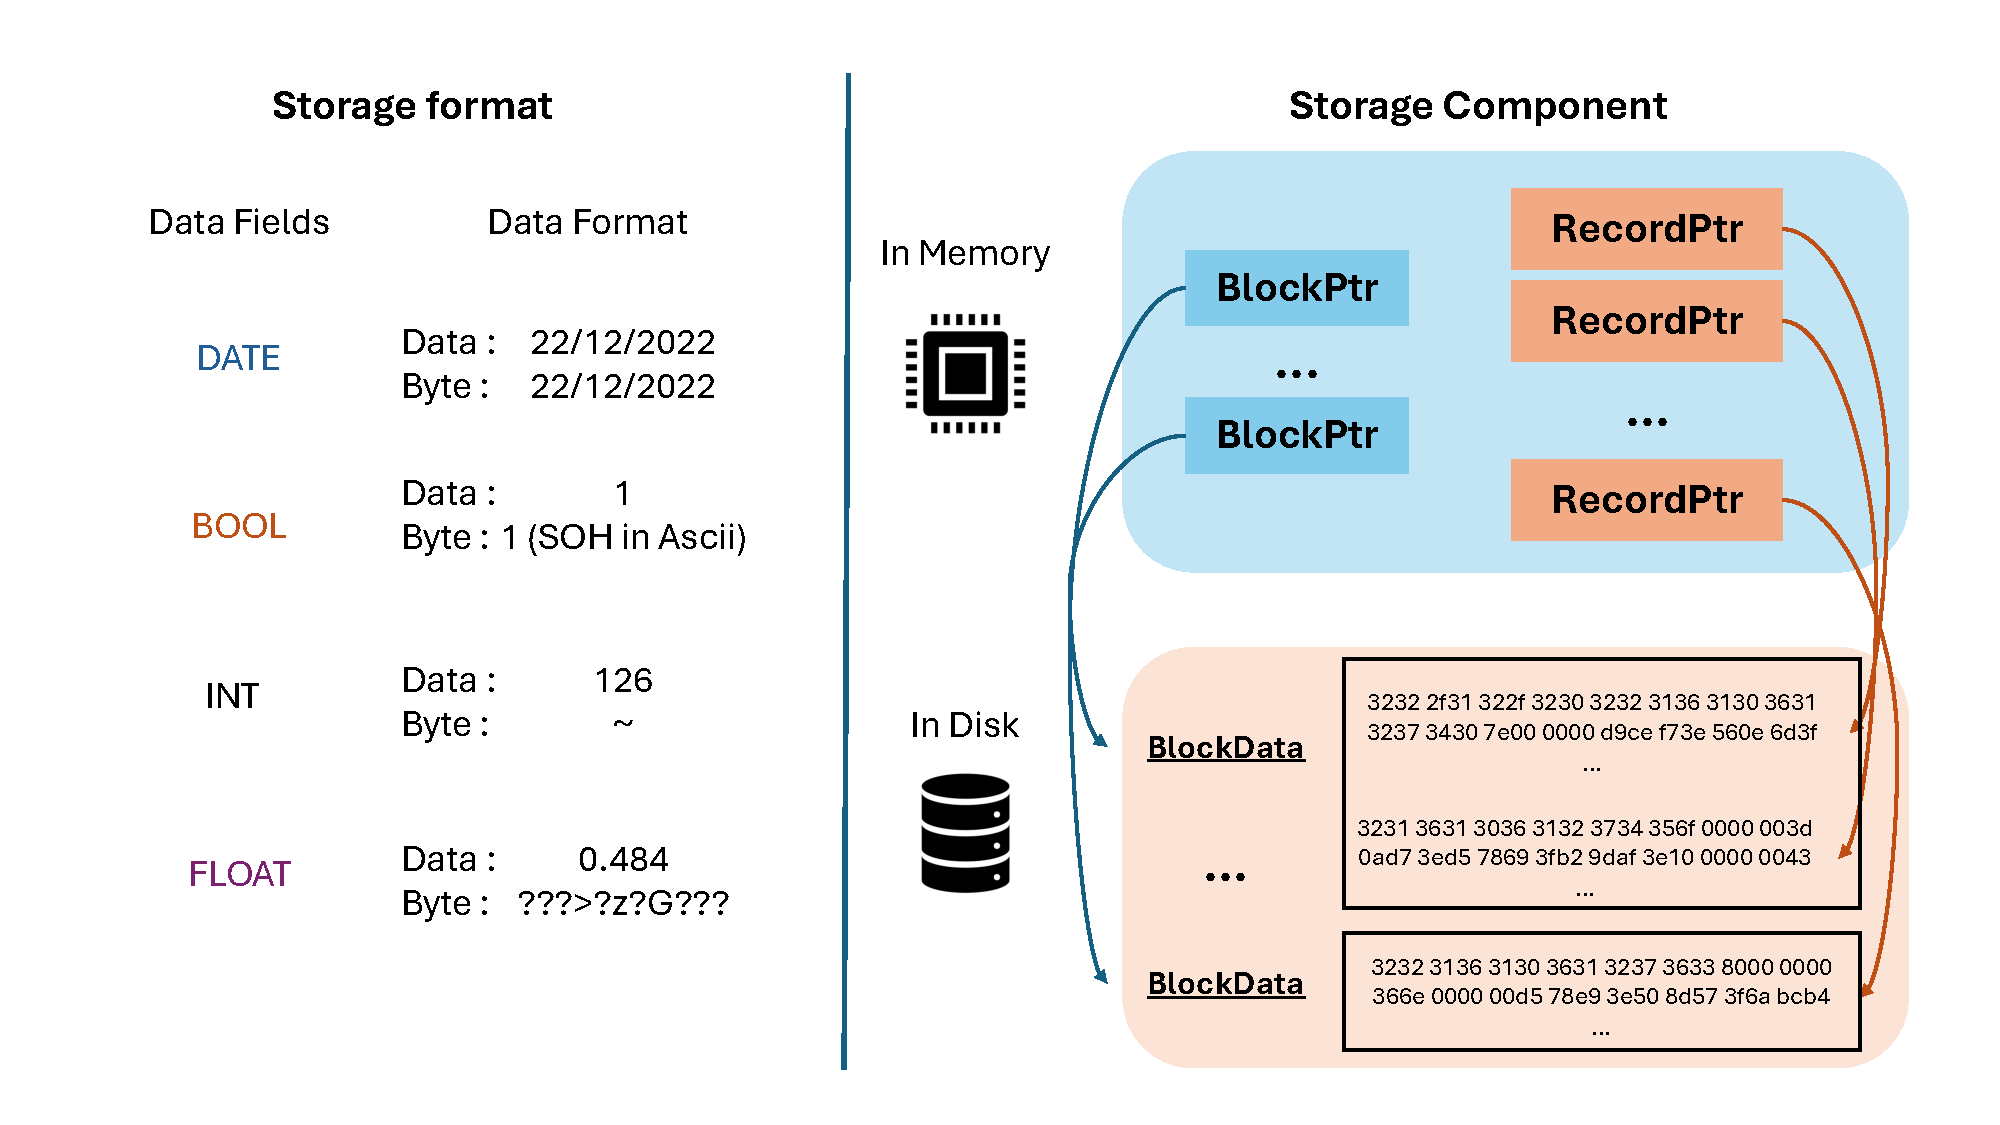
\includegraphics[width=1\linewidth]{figures/Storage_component.pdf}
    \caption{Illustration of the storage components design in our project. All the data are converted into array of Byte and store in the disk. Only pointers that points to the offset position will be stored in memory.}
    \label{fig:storage-component}
\end{figure}


\subsection{Controller Components}
\label{subsec:controller}

\begin{figure}[t]
    \centering
    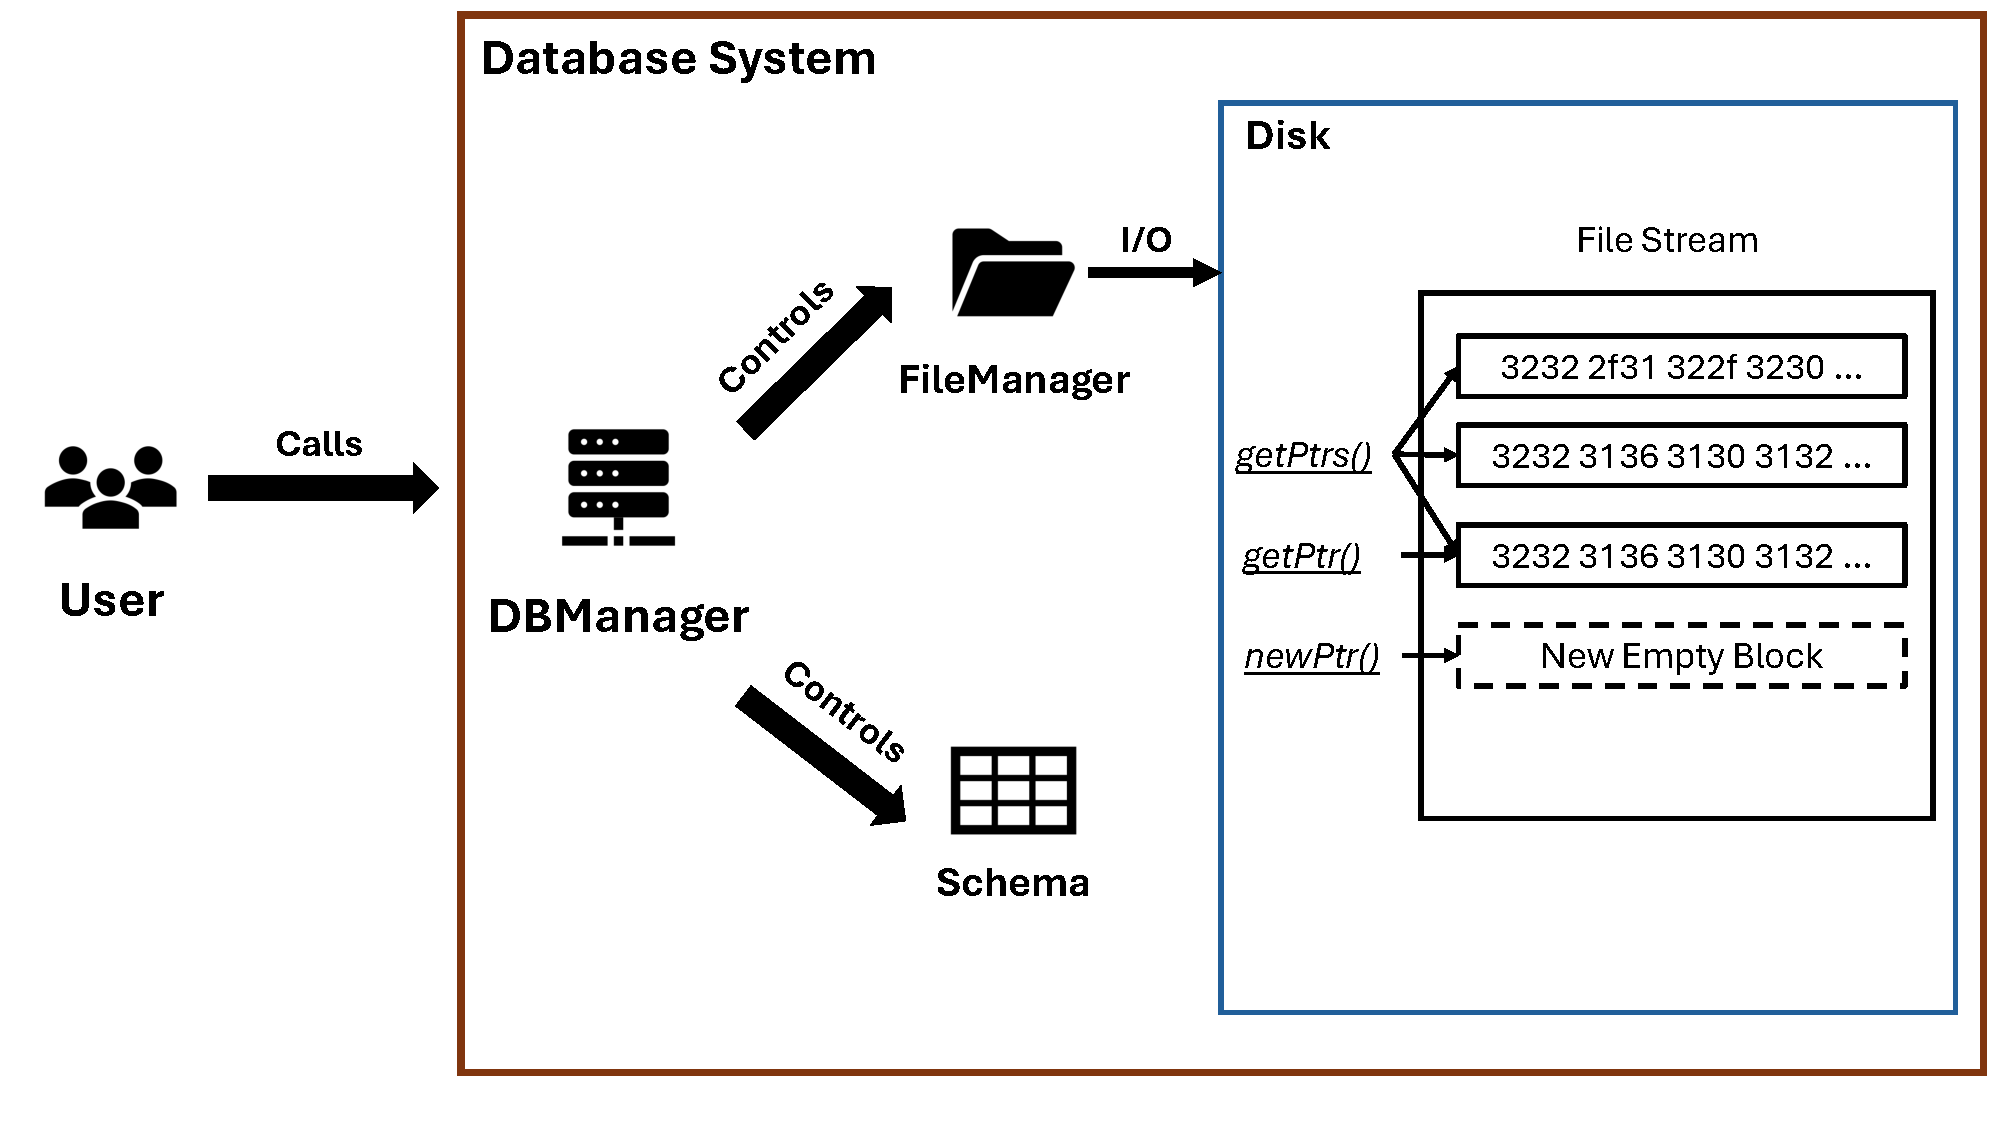
\includegraphics[width=1\linewidth]{figures/Cotroller.pdf}
    \caption{The controller components in how user interactive with the database.}
    \label{fig:Controller}
\end{figure}

We will now illustrate our controller components, which are primarily responsible for managing the data components described in ~\Cref{subsec:data-components}. The two main controller objects are as follows:

\begin{itemize} 
    \item \textbf{FileManager}: This object manages all BlockPtr instances and the file stream. It handles read and write operations between the file and the buffer pool. 
    \item \textbf{DataBaseManager}: This object controls the database, using the FileManager to load data or allocate new memory blocks for data storage. It also oversees the process of reading from the original text file or from the byte array, returning a pointer to the record position. 
\end{itemize}

When interacting with the user, the DataBaseManager calls the FileManager to allocate new memory or read from existing memory. During a \texttt{load()} operation, the DataBaseManager initiates an I/O operation for one block, as detailed in ~\Cref{fig:Controller}.

\subsection{Buffer Pool}
\label{subsec:io-control}

\begin{figure}[ht]
    \centering
    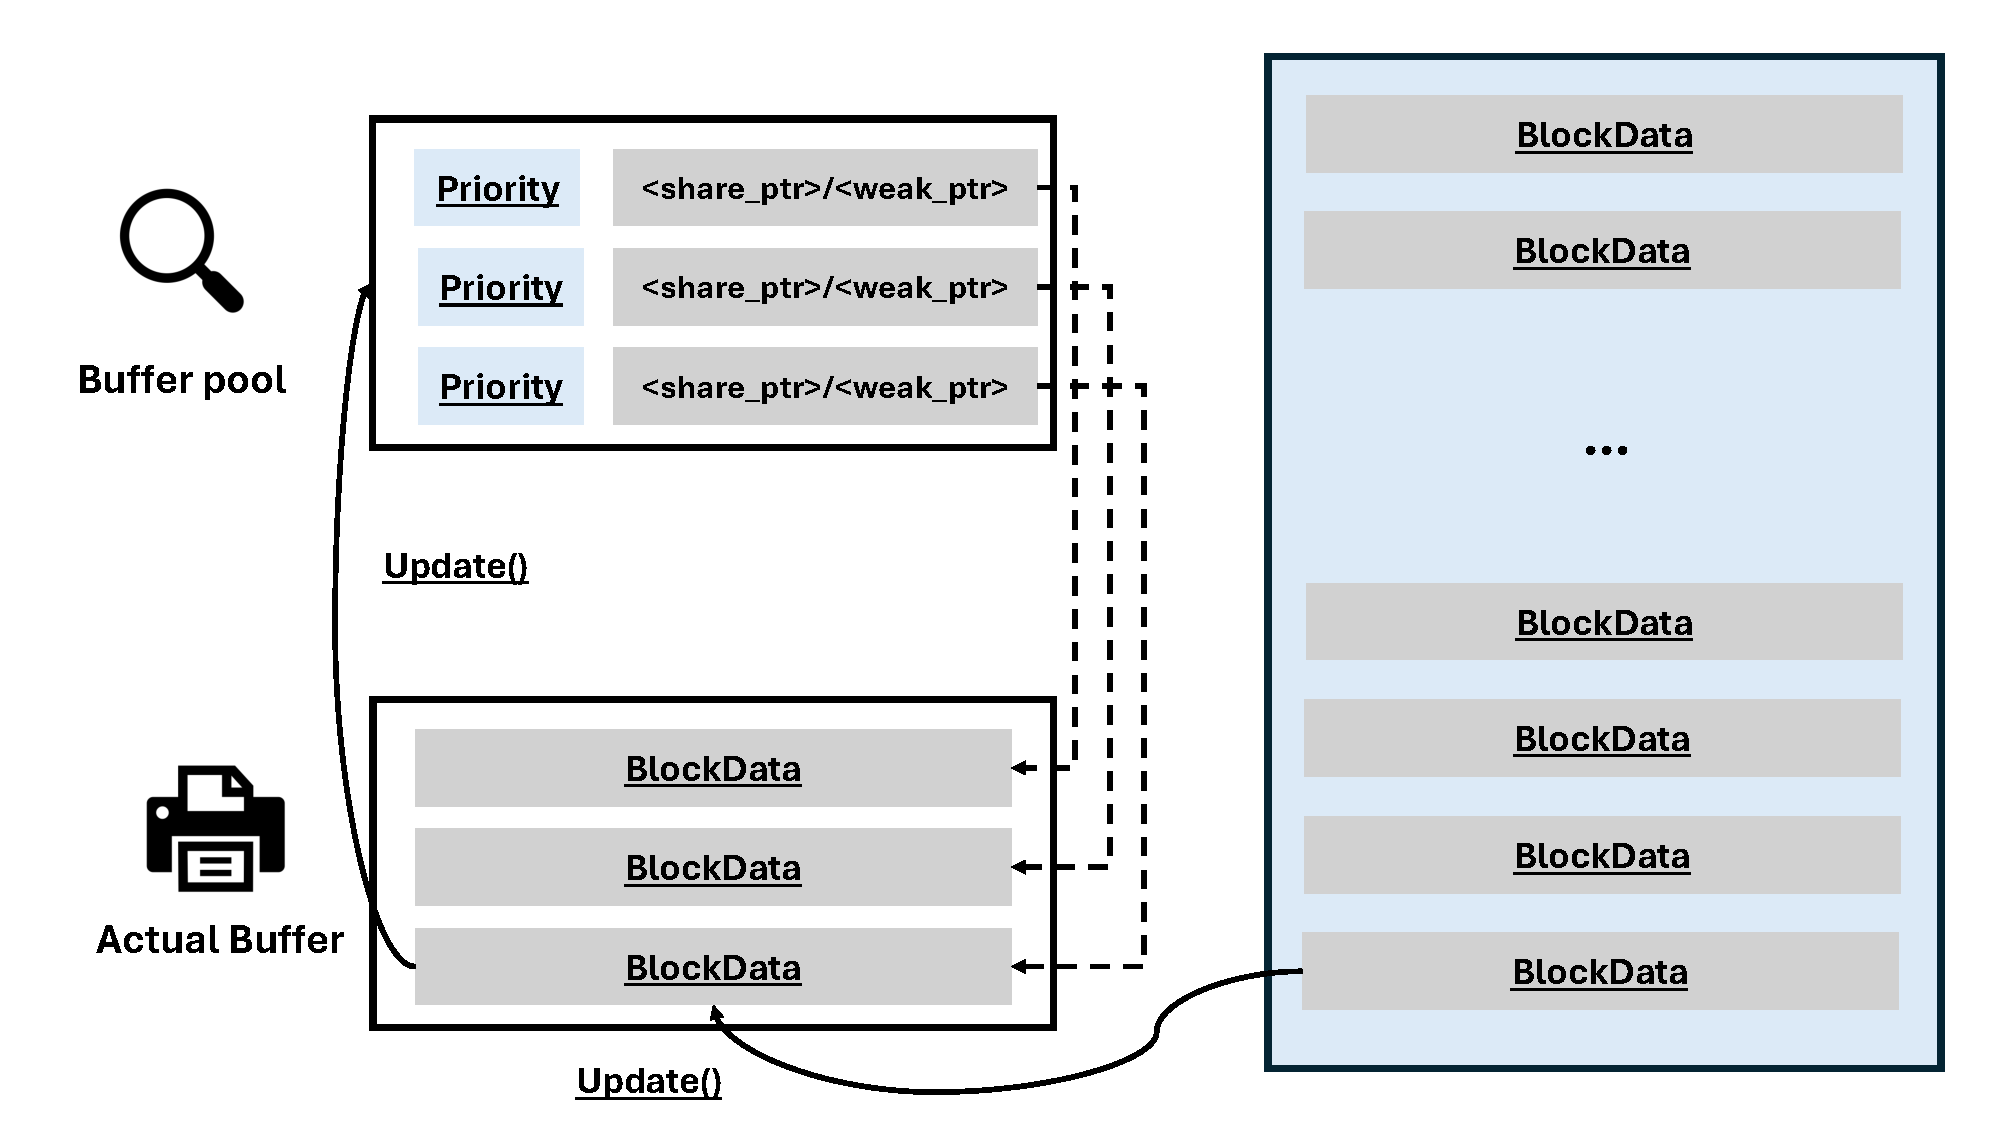
\includegraphics[width=1\linewidth]{figures/Buffer_pool.pdf}
    \caption{Design of our buffer pool. \texttt{BlockData} are shared with \texttt{shared\_ptr} or \texttt{weak\_ptr} so that no duplicate \texttt{BlockData} are constructed. During update, the data in the buffer pool will be override and the index and priority will be update}
    \label{fig:buffer-pool}
\end{figure}

We use the buffer pool to manage disk read and write operations uniformly. All database read and write operations must go through the buffer pool.

A buffer pool $\mathcal{P}$ consists of the following properties:

\begin{enumerate}
    \item A hash table $\mathcal{H}_\mathcal{P}$ in memory, using the disk offset as the key. $\mathcal{H}_\mathcal{P}(o)$ represents the block data corresponding to the disk offset $o$.
    
    \item A Least Recently Used (LRU) queue $\mathcal{Q}_\mathcal{P}$ that tracks the access order of frames, with the least recently used page at the head. This queue implements the page replacement policy in the buffer pool. If the page is replaced in the memory, the block data in the buffer where the old page was stored is expired; when I/O is requested to access the data block corresponding to this buffer, the data block has to be loaded from the memory to this buffer. 
    
    \item Each frame in the buffer pool is associated with a dirty bit $\mathcal{D}$. If $\mathcal{D} = 1$, the frame has been modified in memory but not yet written back to disk. If $\mathcal{D} = 0$, the frame is synchronized with the corresponding block on disk. 
\end{enumerate}

During actual I/O operations, the \texttt{FileManager} manages the buffer and reuses it if the block is already cached in the buffer pool. If the buffer pool is full, it is updated using the \textit{Least Recently Used (LRU)} policy described above. The structure of our buffer pool is illustrated in ~\Cref{fig:buffer-pool}, where each BlockData is shared using \texttt{std::shared\_ptr} or \texttt{std::weak\_ptr} to allow resource sharing. During updates, the data in the buffer is modified accordingly, and the pointers are updated to reflect the changes.

The entire structure simulates the LRU process, achieving $\mathcal{O}(1)$ time complexity for each fetch operation.
